\documentclass[12pt,spanish]{article}

% aprovechamiento de la p\'agina -- fill an A4 (210mm x 297mm) page
% Note: 1 inch = 25.4 mm = 72.27 pt
% 1 pt = 3.5 mm (approx)

% vertical page layout -- one inch margin top and bottom
\topmargin      -10 mm   % top margin less 1 inch
\headheight       0 mm   % height of box containing the head
\headsep          0 mm   % space between the head and the body of the page
\textheight     255 mm   % the height of text on the page
\footskip         7 mm   % distance from bottom of body to bottom of foot

% horizontal page layout -- one inch margin each side
\oddsidemargin    0 mm     % inner margin less one inch on odd pages
\evensidemargin   0 mm     % inner margin less one inch on even pages
\textwidth      159 mm     % normal width of text on page

\usepackage{parskip}

\usepackage{float}

\usepackage[document]{ragged2e}
\usepackage{babel}
\usepackage[utf8]{inputenc}
\usepackage{amsmath,amsthm,mathtools}
\usepackage{amsfonts,amssymb,latexsym}
\usepackage{enumerate}
\usepackage[dvips,usenames]{color}
\definecolor{RojoAnayelRey}{rgb}{1,.25,.25}
\usepackage{tikz}
\usepackage[bookmarks=true,
            bookmarksnumbered=false, % true means bookmarks in 
                                     % left window are numbered                         
            bookmarksopen=false,     % true means only level 1
                                     % are displayed.
            colorlinks=true,
            linkcolor=webred]{hyperref}
\definecolor{webgreen}{rgb}{0, 0.5, 0} % less intense green
\definecolor{webblue}{rgb}{0, 0, 0.5}  % less intense blue
\definecolor{webred}{rgb}{0.5, 0, 0}   % less intense red
\definecolor{dkgreen}{rgb}{0,0.6,0}
\definecolor{gray}{rgb}{0.5,0.5,0.5}
\definecolor{mauve}{rgb}{0.58,0,0.82}
\definecolor{MistyRose}{RGB}{255,228,225}
\definecolor{LightCyan}{RGB}{224,255,255}

%\usepackage{beton}
\usepackage[T1]{fontenc}

% Theorem environments

%% \theoremstyle{plain} %% This is the default
\newtheorem{theorem}{Teorema}[section]
\newtheorem{corollary}[theorem]{Corolario}
\newtheorem{lemma}[theorem]{Lema}
\newtheorem{proposition}[theorem]{Proposici\'on}
%\newtheorem{ax}{Axioma}

\theoremstyle{definition}
\newtheorem{definition}{Definici\'on}[section]
\newtheorem{algorithm}{\textrm{\bf Algoritmo}}[section]

\theoremstyle{remark}
\newtheorem{remark}{Observaci\'on}[section]
\newtheorem{example}{Ejemplo}[section]
\newtheorem{exercise}{Ejercicio}[section]
%\newenvironment{solution}{\begin{proof}[Solution]}{\end{proof}}
\newenvironment{solution}{\begin{proof}[Solución]}{\end{proof}}
\newtheorem*{notation}{Notaci\'on}

%\numberwithin{equation}{section}

%\newcommand{\regla}[2]{
%\begin{array}{c}
%#1\\
%\hline
%#2\\
%\end{array}
%}

\title{Principales resultados de Análisis Vectorial}

\author{David Cabezas Berrido}

\date{}

\begin{document}

\maketitle

Vamos a presentar los principales resultados de la asignatura Análisis Vectorial: el Teorema de Green, el Teorema de la Stokes y el Teorema de la Divergencia. Todos ellos establecen propiedades relativas a las integrales en curvas y superficies de funciones reales de varias variables, normalmente en dimensión 2 y 3.

A continuación, introducimos los conceptos necesarios para la comprensión de cada uno de estos resultados. Seguidamente, iremos presentando los teoremas principales, en cada caso incluiremos una breve explicación intuitiva y un ejemplo donde comprobaremos que se verifica el resultado.

\section{Conceptos previos}

\subsection{Operadores diferenciales}

Los siguientes operadores diferenciales tienen una gran importancia en el análisis real, y algunos de ellos son necesarios para comprender los teoremas antes mencionados.

\subsubsection*{Gradiente}

Sea $f:\Omega\rightarrow\mathbb{R}$ un campo escalar diferenciable, donde $\Omega$ es un abierto de $\mathbb{R}^N$. El \textbf{gradiente} de $f$ es la función $\nabla f: \Omega\rightarrow\mathbb{R}^N$) dada por el vector de derivadas parciales, esto es,
\[\nabla f(x)=\left(\frac{\partial}{\partial x_1}f(x),\ldots,\frac{\partial}{\partial x_1}f(x)\right)\]
para cada $x\in \Omega$.

\subsubsection*{Divergencia}

Si $F:\Omega\rightarrow\mathbb{R}^N$ es un campo vectorial diferencible dado por $F=(F_1,\ldots, F_N)$, la \textbf{divergencia} de $F$ viene dada por
\[\operatorname{div}\big(F(x)\big)=\sum_{i=1}^N\frac{\partial}{\partial x_i}F_i(x).\]
Se tiene $\operatorname{div} F:\Omega\rightarrow\mathbb{R}$.

\subsubsection*{Laplaciano}

Si ahora suponemos que $f$ es de clase 2 ($f\in C^2(\Omega)$), definimos el \textbf{laplaciano} de $f$ como la traza de su matriz Hessiana, es decir, la función $\Delta f:\Omega\rightarrow\mathbb{R}$ dada por
\[\Delta f(x)=\sum_{i=1}^{N}\frac{\partial^2}{\partial x_i^2}f(x).\]
Además, se tiene $\Delta f=\operatorname{div}(\nabla f)$.

\subsubsection*{Rotacional}

Cuando la dimensión es $N=3$, definimos la \textbf{rotacional} del campo vectorial diferenciable $F=(F_1,F_2,F_3)$ como el campo (vectorial) dado por
\[\operatorname{rot F}=\left(\frac{\partial F_3}{\partial x_2}-\frac{\partial F_2}{\partial x_3},\frac{\partial F_1}{\partial x_3}-\frac{\partial F_3}{\partial x_1},\frac{\partial F_2}{\partial x_1}-\frac{\partial F_1}{\partial x_2}\right).\]

Para el caso bidimensional, donde $F=(F_1,F_2)$, tenemos
\[\operatorname{rot F}=\frac{\partial F_2}{\partial x_1}-\frac{\partial F_1}{\partial x_2}.\]
Notemos que en este caso, la rotacional es un campo escalar.

\subsection{Integrales de campos escalares y vectoriales sobre curvas y superficies}

Con la notación anterior, introducimos la forma de integrar campos escalares y vectoriales sobre curvas y superficies.

\subsubsection*{Integral de línea de un campo escalar}

Si $f:\Omega\rightarrow\mathbb{R}$ es un campo escalar continuo con $\Omega\subset\mathbb{R}^N$ y $\gamma:[a,b]\rightarrow\Omega$ es un camino regular a trozos (una función de clase $C^1$ a trozos del intervalo $[a,b]$ en $\Omega$), definimos la \emph{integral de línea de $f$ a lo largo de $\gamma$} como
	\[\int_\gamma f dl=\int_a^b f\big(\gamma(t)\big)\|\gamma'(t)\|dt.\]
	
\subsubsection*{Integral de línea de un campo vectorial}

Si $F:\Omega\rightarrow\mathbb{R}^N$ es un campo escalar continuo con $\Omega\subset\mathbb{R}^N$ y $\gamma:[a,b]\rightarrow\Omega$ es un camino regular a trozos, definimos la \emph{integral de línea de $F$ a lo largo de $\gamma$} como
\[\int_\gamma F dl=\int_a^b \left\langle F\big(\gamma(t)\big),\gamma'(t)\right\rangle dt.\]

\subsubsection*{Integral de superficie de un campo escalar}

Si una superficie $S\subset \mathbb{R}^3$ admite una parametrización simple y suave, para cada función continua $f:S\rightarrow\mathbb{R}$, la \emph{integral de superficie del campo escalar $f$ sobre la superficie $S$} viene definida mediante la igualdad
\[\iint_S f ds=\iint_\Phi f ds=\iint_W f\big(\Phi(u,v)\big)\|\Phi_u\times \Phi_v\| du dv,\]
donde $\Phi:W\rightarrow\mathbb{R}^3$ es cualquier parametrización simple (inyectiva) y suave ($\Phi_u\times \Phi_v$ no se anula en $W$).

Este valor es independiente de la parametrización $\Phi$ elegida.

\subsubsection*{Integral de superficie de un campo vectorial}

Sea $\Phi$ una parametrización simple y suave de $S$ y supongamos que $F:S\rightarrow\mathbb{R}^3$ es una función continua. La \emph{integral de superficie del campo vectorial $F$ sobre la superficie $S$ orientada mediante $\dfrac{\Phi_u\times \Phi_v}{\|\Phi_u\times \Phi_v\|}$} viene dada por la igualdad
\[\iint_S F ds=\iint_\Phi F ds=\iint_W \left\langle F\big(\Phi(u,v)\big), \Phi_u\times \Phi_v\right\rangle du dv.\]

Este valor es independiente de la parametrización $\Phi$ elegida siempre que se respete la misma orientación \Big(siempre que el vector $\dfrac{\Phi_u\times \Phi_v}{\|\Phi_u\times \Phi_v\|}$ sea el mismo\Big). Obtendríamos el valor opuesto si eligiésemos una parametrización simple y suave que determine la orientación opuesta. Esto depende de si el vector $\dfrac{\Phi_u\times \Phi_v}{\|\Phi_u\times \Phi_v\|}$ es normal exterior o interior a la superficie.

\section{Teorema de Green}

El Teorema de Green asegura que el valor de la integral de línea de un campo vectorial de clase $C^1$ y dimensión 2 a lo largo de una curva de Jordan viene determinado por la integral doble de su rotacional en la región interior a la curva. 

\begin{theorem}[Teorema de Green]
	Sea $\gamma$ un camino en $\mathbb{R}^2$, regular a trozos, cerrado y simple, que recorre una curva de Jordan $\Gamma$ en sentido positivo (antihorario). Sea $D$ la región interior a $\Gamma$, y $F=(F_1,F_2):\Omega\rightarrow\mathbb{R}^2$ un campo vectorial de clase $C^1$ en un abierto $\Omega\subset\mathbb{R}^2$ tal que $D\cup\Gamma\subset\Omega$. Entonces,
	\[\int_\gamma F dl = \iint_D \operatorname{rot}F dA.\]
\end{theorem}

Más explícitamente, esto puede escribirse como
\[\int_\gamma F_1 dx+F_2 dy=\iint_D \left(\frac{\partial F_2}{\partial x}-\frac{\partial F_1}{\partial y}\right) dx dy.\]

\subsection*{Ejemplo}

Comprobemos ahora el Teorema de Green en un ejemplo concreto.

Consideremos el campo vectorial $F:\mathbb{R}^2\rightarrow\mathbb{R}^2$ dado por $F(x,y)=(x+2y,3x-5y)$, y la región $D=\{(x,y)\in\mathbb{R}^2: x^2+4y^2\leq 4\}$.

Tenemos $F_1(x,y)=x+2y$ y $F_2(x,y)=3x-5y$, por tanto
\[\operatorname{rot}F=\frac{\partial F_2}{\partial x}-\frac{\partial F_1}{\partial y}=3-2=1.\]

Por una parte, la integral en $D$ de la función constante 1 coincide con el área de $D$. $D$ es el área encerrada por una elipse centrada en el origen con ejes de longitud $2$ y $1$.

\begin{figure}[H]
	\centering
	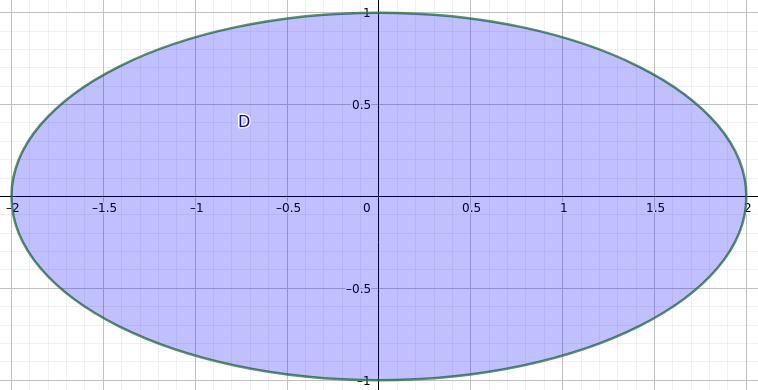
\includegraphics[width=120mm]{images/region-ejemplo-green}
\end{figure}

El área de una elipse cuyos ejes tienen longitud $a$ y $b$ es $\pi a b$, por tanto el área de $D$ es $\pi\cdot1\cdot 2=2\pi$.

Por tanto, $\displaystyle{\iint_D \operatorname{rot}F dx dy}=2\pi$.

Para la otra integral, parametrizamos la elipse que encierra a $D$ con la curva $\gamma:[0,2\pi]\rightarrow\mathbb{R}^2$ dada por $\gamma(t)=(2\cos t, \sin t)$.

\begin{figure}[H]
	\centering
	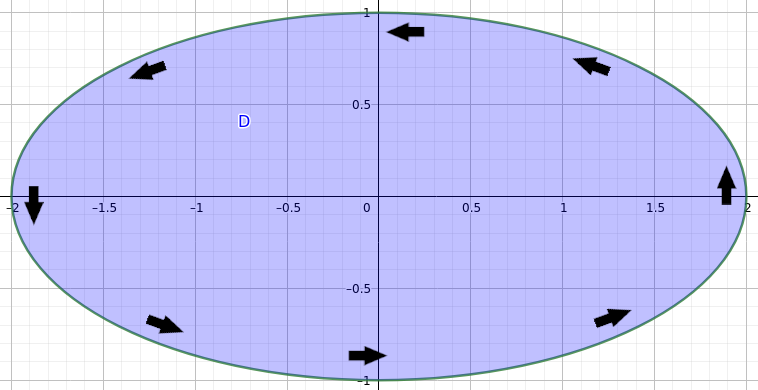
\includegraphics[width=120mm]{images/region-ejemplo-green-flechas}
\end{figure}

Tenemos $\gamma'(t)=(-2\sin t, \cos t)$, y la integral queda entonces:
\[\int_\gamma F dl = \int_0^{2\pi}\left\langle F\big(\gamma(t)\big),\gamma'(t)\right\rangle dt=\int_0^{2\pi}\left\langle (2\cos t+2\sin t,6\cos t-5\sin t),(-2\sin t, \cos t)\right\rangle dt.\]
Simplificando obtenemos
\[\int_\gamma F dl=-4\int_0^{2\pi}\sin^2 t dt +6\int_0^{2\pi}\cos^2 t dt=-4\pi+6\pi=2\pi,\]
y comprobamos que se verifica el Teorema de Green.

\section{Teorema de la Divergencia en $\mathbb{R}^2$}

El Teorema de la Divergencia permite, dado un campo vectorial, calcular fácilmente el flujo saliente de una región. El flujo saliente se expresa como la integral del producto escalar entre el campo y la normal exterior a la frontera (curva, superficie o hipersuperficie) del recinto a lo largo de la frontera. Gracias a este teorema, podemos obtener el flujo saliente integrando la divergencia del campo (que es una función escalar) en la región del espacio.

\begin{theorem}[Teorema de la Divergencia en $\mathbb{R}^2$]
	Sea $\Omega$ un dominio de $\mathbb{R}^2$ y $F=(F_1,F_2):\Omega\rightarrow\mathbb{R}^2$ un campo vectorial de clase $C^1$.
	Sea $\Gamma\subset\Omega$ una curva de Jordan $C^1$ a trozos orientada positivamente, y $D$ la región interior a $\Gamma$. Tomamos la normal exterior a $\Gamma$. Esto es, si $\gamma(t)=(x(t),y(t))$ es una parametrización que recorre $\Gamma$ en el sentido positivo y $\gamma'(t)=(x'(t),y'(t))$, la normal exterior a $\Gamma$ es $n(t)=\dfrac{(y'(t),-x'(t))}{\|\gamma'(t)\|}$. Entonces, 
	\[\int_\Gamma \langle F,n\rangle dl=\iint_D\operatorname{div} F dA=\iint_D\left(\frac{\partial F_1}{\partial x}+\frac{\partial F_2}{\partial y}\right) dx dy.\]
\end{theorem}

\begin{proof}
	Utilizando la definición de integral curvilínea de un campo escalar y desarollando el producto obtenemos
	\begin{align*}
	\int_\Gamma \langle F,n\rangle dl&=\int_a^b\frac{F_1\big(\gamma(t)\big)y'(t)-F_2\big(\gamma(t)\big)x'(t)}{\|\gamma'(t)\|}\|\gamma'(t)\|dt \\
	&=\int_a^b F_1\big(\gamma(t)\big)y'(t)-F_2\big(\gamma(t)\big)x'(t)dt = \int_a^bF_1\big(\gamma(t)\big)dy-F_2\big(\gamma(t)\big)dx \\
	&=\int_\Gamma F_1 dy-F_2dx.
	\end{align*}
	Finalmente, el Teorema de Green aplicado al campo $(-F_2,F_1)$ nos asegura que 
	\[\int_\Gamma \langle F,n\rangle dl=\int_\Gamma F_1 dy-F_2dx=\iint_D\left(\frac{\partial F_1}{\partial x}+\frac{\partial F_2}{\partial y}\right) dx dy.\]
\end{proof}

\subsection*{Ejemplo}

Comprobemos que este teorema se verifica en el ejemplo anterior, con el campo $F(x,y)=x+2y,3x-5y$ y la región $D=\{(x,y)\in\mathbb{R}^2: x^2+4y^2\leq 4\}$.

Por una parte, tenemos $\operatorname{div}F=1-5=-4$, y el resultado de integrar en $D$ es el mismo que obtenemos multiplicando por el área:
\[\iint_D\operatorname{div} F dA= -4\cdot 2\pi=-8\pi.\]

Por otra parte, utilizaremos la misma parametrización que recorre la curva en sentido positivo, $\gamma:[0,2\pi]\rightarrow\mathbb{R}^2$ con $\gamma(t)=(2\cos t, \sin t)$. Tenemos $\gamma'(t)=(-2\sin t, \cos t)$, luego $n(t)=\dfrac{(\cos t,2\sin t)}{\sqrt{\cos^2 t+4\sin^2 t}}$.

Desarrollando obtenemos:
\begin{align*}
\int_\Gamma \langle F,n\rangle dl&=\int_0^{2\pi} \left\langle F(2\cos t, \sin t),\frac{(\cos t,2\sin t)}{\sqrt{\cos^2 t+4\sin^2 t}}\right\rangle\sqrt{\cos^2 t+4\sin^2 t} dt \\
&=\int_0^{2\pi} \langle (2\cos t+2\sin t,6\cos t-5\sin t),(\cos t,2\sin t)\rangle dt.
\end{align*}

Ahora simplificamos, lo que nos deja con

\[\int_\gamma F dl=2\int_0^{2\pi}\cos^2 t dt -10\int_0^{2\pi}\sin^2 t dt =2\pi-10\pi=-8\pi,\]
y comprobamos que se verifica el Teorema de la Divergencia en este caso.

\section{Teorema de Stokes}

El Teorema de Stokes es una generalización del Teorema de Green, que permite obtener la misma tesis para superficies que tienen curvas alabeadas como bordes, en lugar de para regiones del plano con curvas planas como bordes. Por tanto, trabajaremos en dimensión 3.

\begin{theorem}[Teorema de Stokes]
	Sea $S$ una superficie orientada definida mediante una parametrización simple y suave $\Phi:D\rightarrow S$, donde $D$ es una región del plano verificando las hipótesis del Teorema de Green (su frontera es una curva de Jordan regular a trozos). Sea $\partial S=\Phi(\partial D)$ la frontera de $S$ con la orientación positiva (inducida por $\Phi$). Sea $F$ un campo vectorial de clase $C^1$ en un abierto que contine a $S$. Entonces,
	\[\iint_S \operatorname{rot}F ds=\int_{\partial S} F dl.\]
\end{theorem}

\begin{proof}
	Supondremos que $S$ es la gráfica de una función, $S=\{(x,y,f(x,y)): (x,y)\in D\}$ con $f\in C^2(D)$. En este caso, $\partial S=\{(x,y,f(x,y)): (x,y)\in \partial D\}$.
	
	Sea $c:[a,b]\rightarrow \partial D$, $c(t)=(x(t),y(t))$ una parametrización en el sentido positivo de $\partial D$. Entonces, $p:[a,b]\rightarrow \partial S$, $p(t)=\big(x(t),y(t),f(x(t),y(t))\big)$ es una parametrización en el sentido positivo de $\partial S$.
	
	Si $F=(F_1,F_2,F_3)$ con $F_1,F_2,F_3\in C^1$, tenemos
	\[\operatorname{rot F}=\left(\frac{\partial F_3}{\partial y}-\frac{\partial F_2}{\partial z},\frac{\partial F_1}{\partial z}-\frac{\partial F_3}{\partial x},\frac{\partial F_2}{\partial x}-\frac{\partial F_1}{\partial y}\right).\]
	
	$S$ es la gráfica de una función, luego su vector perpendicular \big($\Phi_x\times \Phi_y$ para la parametrización $\Phi(x,y)=(x,y,f(x,y))$\big) en el punto $(x,y,z=f(x,y))$ es $(-z_x,-z_y,1)$. Por tanto,
	\begin{align*}
	\iint_S \operatorname{rot}F ds=\iint_D -z_x\left(\frac{\partial F_3}{\partial y}-\frac{\partial F_2}{\partial z}\right) -z_y\left(\frac{\partial F_1}{\partial z}-\frac{\partial F_3}{\partial x}\right)+\frac{\partial F_2}{\partial x}-\frac{\partial F_1}{\partial y} dx dy.
	\end{align*}
	
	Por otra parte,
	\begin{align*}
	\int_{\partial S} F dl=\int_a^b \big(F_1 x'(t) + F_2 y'(t) + F_3 z'(t)\big) dt,
	\end{align*}
	y aplicando que $z'(t)=\dfrac{\partial z}{\partial x}\dfrac{d x}{d t}+\dfrac{\partial z}{\partial y}\dfrac{d y}{d t}$, obtenemos
	\begin{align*}
	\int_{\partial S} F dl&=\int_a^b\left[\left(F_1+F_3\dfrac{\partial z}{\partial x}\right)\dfrac{d x}{d t}+\left(F_2+F_3\dfrac{\partial z}{\partial y}\right)\dfrac{d y}{d t}\right]dt \\
	&=\int_a^b\left(F_1+F_3\dfrac{\partial z}{\partial x}\right)d x+\left(F_2+F_3\dfrac{\partial z}{\partial y}\right)d y.
	\end{align*}
	
	Aplicamos el Teorema de Green al campo $\left(F_1+F_3\dfrac{\partial z}{\partial x},F_2+F_3\dfrac{\partial z}{\partial y}\right)$:
	\begin{align*}
	\int_{\partial S} F dl=\iint_D\left[\frac{d}{d x}\left(F_2+F_3\dfrac{\partial z}{\partial y}\right)-\frac{d}{d y}\left(F_1+F_3\dfrac{\partial z}{\partial x}\right)\right]dA.
	\end{align*}
	
	Ahora desarrollamos, debemos tener en cuenta que $F_1,F_2,F_3$ dependen de 3 variables: $x,y,z$, pero a su vez la variable $z=f(x,y)$ depende de las dos primeras.
	\begin{align*}
	\int_{\partial S} F dl&=\iint_D\left[\frac{d F_2}{d x}+\frac{d F_3}{d x}\dfrac{\partial z}{\partial y}+F_3\frac{\partial^2 z}{\partial x\partial y}-\frac{d F_1}{d y}-\frac{d F_3}{d y}\dfrac{\partial z}{\partial x}\right]dA \\
	&=\iint_D\bigg[\frac{\partial F_2}{\partial x}+\frac{\partial F_2}{\partial z}\frac{\partial z}{\partial x}+\left(\frac{\partial F_3}{\partial x}+\frac{\partial F_3}{\partial z}\frac{\partial z}{\partial x}\right)\dfrac{\partial z}{\partial y}+F_3\frac{\partial^2 z}{\partial x\partial y} \\
	 &~\hspace{10mm}-\frac{\partial F_1}{\partial y}-\frac{\partial F_1}{\partial z}\frac{\partial z}{\partial y}-\left(\frac{\partial F_3}{\partial y}+\frac{\partial F_3}{\partial z}\frac{\partial z}{\partial y}\right)\dfrac{\partial z}{\partial x}-F_3\frac{\partial^2 z}{\partial y\partial x}\bigg]dA.
	\end{align*}
	Usamos que $F_3\in C^2$ para simplificar y sacamos factor común las derivadas parciales de $z$ con signo negativo y el $1$. Obtenemos así la conclusión deseada.
		\begin{align*}
	\int_{\partial S} F dl&=\iint_D\bigg[\frac{\partial F_2}{\partial x}+\frac{\partial F_2}{\partial z}\frac{\partial z}{\partial x}+\frac{\partial F_3}{\partial x}\dfrac{\partial z}{\partial y}-\frac{\partial F_1}{\partial y}-\frac{\partial F_1}{\partial z}\frac{\partial z}{\partial y}-\frac{\partial F_3}{\partial y}\dfrac{\partial z}{\partial x}\bigg]dA \\
	&=\iint_D\bigg[-\frac{\partial z}{\partial x}\left(\frac{\partial F_3}{\partial y}-\frac{\partial F_2}{\partial z}\right)-\dfrac{\partial z}{\partial y}\left(\frac{\partial F_1}{\partial z}-\frac{\partial F_3}{\partial x}\right)+\frac{\partial F_2}{\partial x}-\frac{\partial F_1}{\partial y}\bigg]dA\\
	&=\iint_S \operatorname{rot}F ds.
	\end{align*}
	
\end{proof}

\subsection*{Ejemplo}

Comprobemos el teorema en un sencillo ejemplo concreto. Consideremos el campo $F(x,y)=(x-y+z,2x+y,y+6z)$ y la superficie \[S=\big\{(x,y,z)\in\mathbb{R}^3: x^2+y^2\leq 1, \  z=\sqrt{1-x^2-y^2}\big\},\]
que corresponde a la mitad superior de la esfera unidad.

El borde de la superficie es la circunferencia unidad en el plano $\{(x,y,0):x,y\in\mathbb{R}\}$. Lo parametrizamos con la curva $\gamma(t)=(\cos t,\sin t, 0)$ con $t\in[0,2\pi]$, cuya derivada es $\gamma'(t)=(-\sin t, \cos t, 0)$. De modo que la integral de línea queda:
\begin{align*}
\int_{\partial S} F dl&=\int_0^{2\pi}\langle F(\cos t,\sin t, 0),(-\sin t, \cos t, 0) \rangle dt \\ 
&=\int_0^{2\pi} -\sin t (\cos t-\sin t+0)+\cos t (2\cos t+\sin t)dt \\
&=\int_0^{2\pi} \sin^2 t + 2\cos^2t \ dt = 3\pi.
\end{align*}

Para la integral sobre la superficie, la parametrizamos de la siguiente forma:
\begin{gather*}
(\rho,\theta)\in[0,1]\times[0,2\pi];\quad (x,y,z)=\Phi(\rho,\theta)=\big(\rho\cos \theta, \rho\sin\theta, \sqrt{1-\rho^2}\big).
\end{gather*}
Calculamos el vector $\Phi_\rho\times \Phi_\theta=\left(\cos\theta,\sin\theta,\frac{-\rho}{\sqrt{1-\rho^2}}\right)\times (-\rho\sin\theta,\rho\cos\theta,0)$ haciendo el producto vectorial y obtenemos
\[\Phi_\rho\times \Phi_\theta=\left(\frac{\rho^2\cos\theta}{\sqrt{1-\rho^2}},\frac{\rho^2\sin\theta}{\sqrt{1-\rho^2}},\rho\right)=\frac{\rho}{\sqrt{1-\rho^2}}\Phi(\rho,\theta).\]

Tenemos también $\operatorname{rot} F=(1-0,1-0,2-(-1))=(1,1,3)$.

La integral de superficie queda entonces:
\begin{align*}
\iint_{S}\operatorname{rot} F dl&=\int_0^1\int_0^{2\pi}\frac{\rho}{\sqrt{1-\rho^2}}\left\langle(1,1,3),\big(\rho\cos \theta, \rho\sin\theta, \sqrt{1-\rho^2}\big)\right\rangle d\theta d\rho \\ 
&=\int_0^1\int_0^{2\pi}\frac{\rho}{\sqrt{1-\rho^2}}\left[\rho\cos\theta+\rho\sin\theta+3\sqrt{1-\rho^2} \right] d\theta d\rho \\
&= 6\pi\int_0^1 \rho d\rho=3\pi.
\end{align*}
Como era de esperar, ambas integrales coinciden.

\section{Teorema de la Divergencia en $\mathbb{R}^N$}

\subsection{Preámbulo}

TODO: dominio regular (se puede hablar de normal exterior a la frontera).

En un regular se puede despejar en la frontera una componente en función de las demás.

Particiones continuas de la unidad, caso compacto (cierre de acotado)

\subsection{Resultado pricipal}

TODO: pag 26

\end{document}

